\documentclass[9pt, aspectratio=169]{beamer}
\usetheme{metropolis}
\usepackage{FiraSans}
\usefonttheme[onlymath]{serif}
\usepackage[utf8]{inputenc}
\usepackage{amsmath}
\usepackage{amsfonts}
\usepackage{amssymb}
\usepackage{multicol}
\usepackage{tikz}
\usepackage{graphicx}
\usepackage{color}
\usepackage[T1]{fontenc} 
\usepackage[skins]{tcolorbox}
\author{Nicola Roman\`o - nicola.romano@ed.ac.uk}
\title{Image preprocessing}
\setlength{\fboxsep}{0pt}
\setbeamertemplate{caption}{\raggedright\insertcaption\par}
\setbeamertemplate {footline}{\begin{scriptsize}\hfill\insertframenumber ~of \inserttotalframenumber\kern1em\vskip5pt\end{scriptsize}}

%\setbeamercovered{transparent} 
%\setbeamertemplate{navigation symbols}{} 

\titlegraphic{\centering 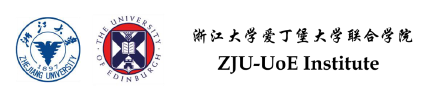
\includegraphics[scale=.5]{instituteLogo.png}}
%\institute{} 
\date{}
%\subject{} 

\begin{document}

\newtcolorbox{codebox}{enhanced,
	top=2pt,
	left=2pt,
	right=2pt,
	bottom=2pt,
	boxrule=0pt,
	leftrule=5pt,
	sharp corners,
	colback=gray!20,
	colframe=blue!60!black}

\begin{frame}
	\maketitle
\end{frame}

\begin{frame}
	{Learning objectives}
	At the end of this lecture you will be able to:

	\begin{itemize}
		\item Give examples of preprocessing in image analysis
		\item Explain basic preprocessing operations such as cropping, resizing, histogram manipulation and filtering
		\item Perform such operations using Python
	\end{itemize}
\end{frame}

\begin{frame}
	{A general quantitative image processing pipeline}

	When analysing a set of images you will need to process them to go from raw data to an output.

	\begin{figure}
		\centering
		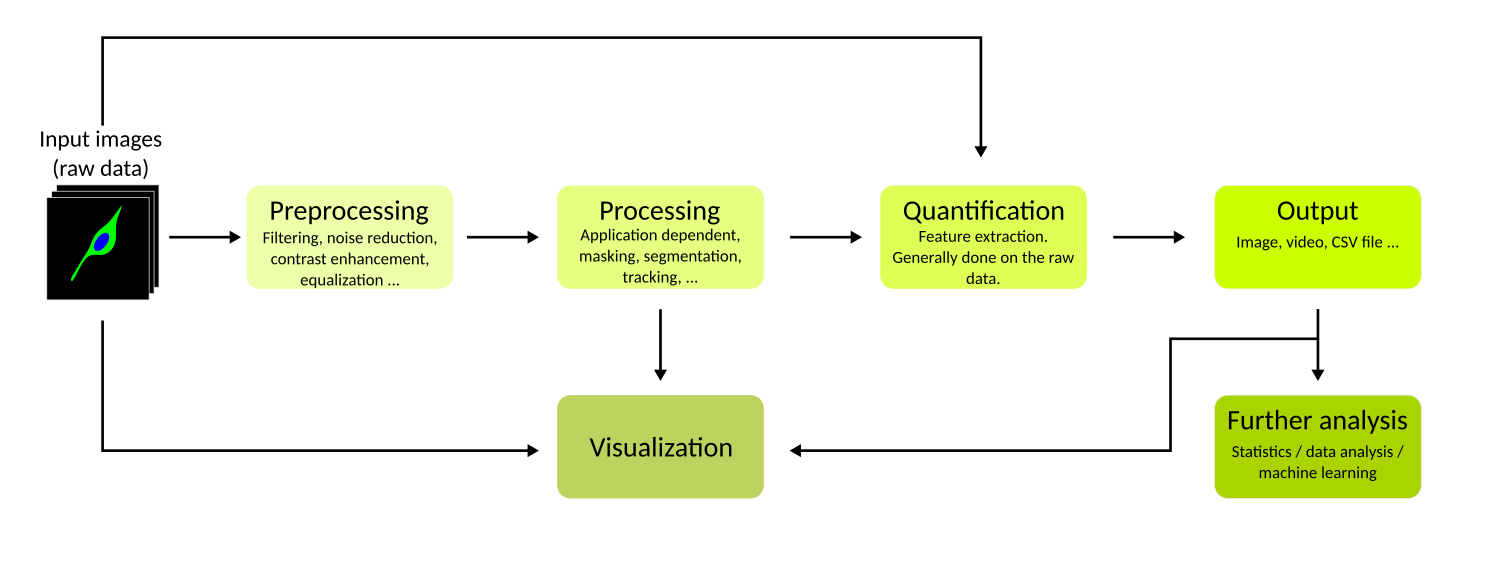
\includegraphics[width=\textwidth]{pipeline.png}
	\end{figure}

\end{frame}

\begin{frame}
	{What is preprocessing?}
	Preprocessing is a series of operations done on input images to improve their quality, suppress unwanted features such as noise, standardise or enhance them to improve further processing operations.

	Preprocessing can happen at the pixel level (e.g. changing intensity) or at the whole image level (e.g. changing size).

	It's important to always \textbf{keep your raw images} and to be aware of possible distortions in your data due to preprocessing (i.e. be sure to know what you are doing!)
\end{frame}

\begin{frame}
	{Why preprocessing?}
	\begin{itemize}
		\item
		      \begin{multicols*}{2}
			      You run an image-classification task to identify whether your image contains normal or cancer tissue. You decide to use a neural network to do so, but your images are all different sizes.\\
			      \columnbreak
			      \textbf{Preprocessing:} you crop/rescale images so that they are all the same size.

			      \centering
			      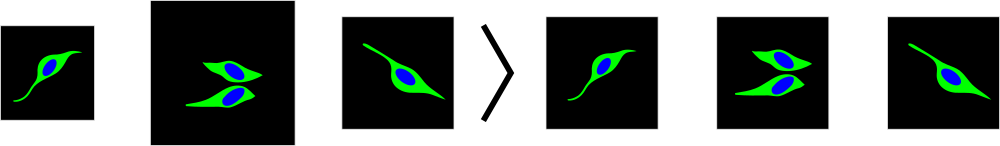
\includegraphics[width=0.5\textwidth]{preproc_example1.png}
		      \end{multicols*}
		      \pause
		\item
		      \begin{multicols*}{2}
			      You want to detect the outline of cells in a series of images (segmentation). Some of your images are undersaturated.\\
			      \columnbreak
			      \textbf{Preprocessing:} you normalise the intensity in all of the images to be between 0 and max (e.g. 0 and 255 for an 8-bit image).

			      \centering
			      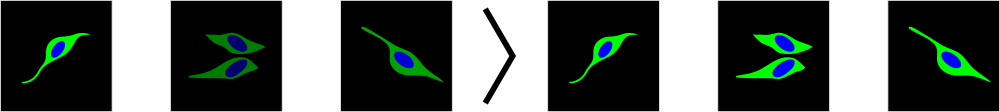
\includegraphics[width=0.5\textwidth]{preproc_example2.png}
		      \end{multicols*}
		      \pause
		\item
		      \begin{multicols*}{2}
			      You are analysing a set of automatically-acquired images from high-throughput screening. Some images are out of focus.\\
			      \columnbreak
			      \textbf{Preprocessing:} you automatically remove out-of-focus images (not easy!).

			      \centering
			      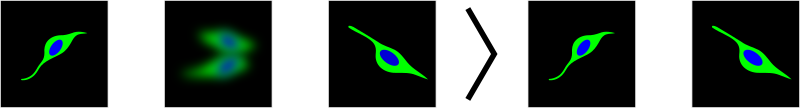
\includegraphics[width=0.4\textwidth]{preproc_example3.png}
		      \end{multicols*}

	\end{itemize}
\end{frame}

\begin{frame}
	{Your toolkit}
	There are countless tools to process images, each with its strength and weaknesses.

	For this task, your \textit{best friends} in Python are (this is not a complete list)

	\begin{itemize}
		\item \textbf{\color{orange}{Numpy}} (see previous lecture) to deal with matrices
		\item \textbf{\color{orange}{Scikit Image}} and \textbf{OpenCV} for image processing
		\item \textbf{\color{orange}{Matplotlib}} for visualization
		\item \textbf{Pandas} for dealing with data frames
		\item \textbf{Scikit Learn} for machine learning (ML)
		\item \textbf{Keras} for advanced ML (convolutional neural network)
	\end{itemize}
\end{frame}

\begin{frame}
	{Scikit Image}
	\begin{figure}
		\centering
		
\includegraphics[width=.5\textwidth]{skimage.png}
	\end{figure}
	\textbf{Scikit Image} is an open-source collection of algorithms for image processing.

	Note that the official name of the library (e.g. for installing it using pip) is \textit{scikit-image}. When you import it in a script you must use \texttt{import skimage})

	\pause
	There are many submodules in Scikit Image that allow performing from simple to very complex operations on images. We will use some of the modules today, the full list can be found in the \href{https://scikit-image.org/docs/stable/api/api.html}{\underline{scikit-image documentation}}.

\end{frame}

\begin{frame}
	{Image cropping}
	Image cropping is very easy using Numpy, just select the part of the image you want to take.

	\begin{codebox}
		\texttt{from skimage.io import imread\\
			img = imread("cells.tif")\\
			print(img.shape) \# (256, 256)\\
			\pause
			img\_cropped = img[50:150, 60:160]\\
			print(img\_cropped.shape) \# (100, 100)\\
			\pause
			\# Also works in multiple dimensions\\
			movie = imread("cellsmovie.tif") \# shape (1000, 256, 256)\\
			movie\_start = img
				[1:100] \# First 100 frames only\\
			\pause
			\# Note that time could have been on axis 2!\\
			\# In that case shape would have been (256, 256, 1000)\\
			\# You would have used img[:, :, 1:100]
		}
	\end{codebox}

	\only<5>
	{
		Cropping is a lossy operation. You \textbf{will lose information} from your original image, so proceed with caution.
	}
\end{frame}

\begin{frame}
	{Image resizing}
	When resizing an image the number of pixel in the output will differ from the input.

	How to account for \textit{lost} pixels when down-scaling or for \textit{missing} pixels when up-scaling? \textbf{Interpolation!}

	\pause
	\begin{figure}
		\centering
		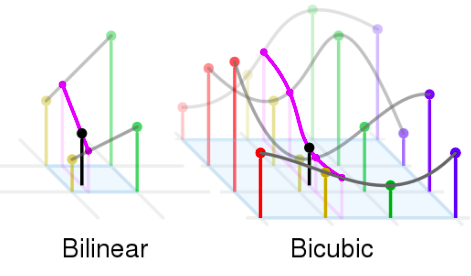
\includegraphics[width=.5\textwidth]{interpolations.png}
	\end{figure}
\end{frame}

\begin{frame}
	{Image resizing - skimage}
	We can use \textit{skimage.transform} to rescale an image.

	\only<1>{Three functions are available:

		\begin{itemize}
			\item \textbf{rescale} -> to scale up/down by a certain factor
			\item \textbf{resize} -> to scale up/down to a certain size
			\item \textbf{downscale\_local\_mean} -> downscale with local averaging
		\end{itemize}
	}

	\only<2>{\begin{codebox}
			\texttt{from skimage.transform import rescale\\
				smiley = imread("smiley.png")\\
				fig, ax = plt.subplots(1, 4)\\
				ax[0].imshow(smiley, cmap="gray")\\
				ax[1].imshow(rescale(smiley, 3, order=0), cmap="gray")\\
				ax[2].imshow(rescale(smiley, 3, order=1), cmap="gray")\\
				ax[3].imshow(rescale(smiley, 3, order=2), cmap="gray")\\
				plt.show()}
		\end{codebox}
		\begin{figure}
			\centering
			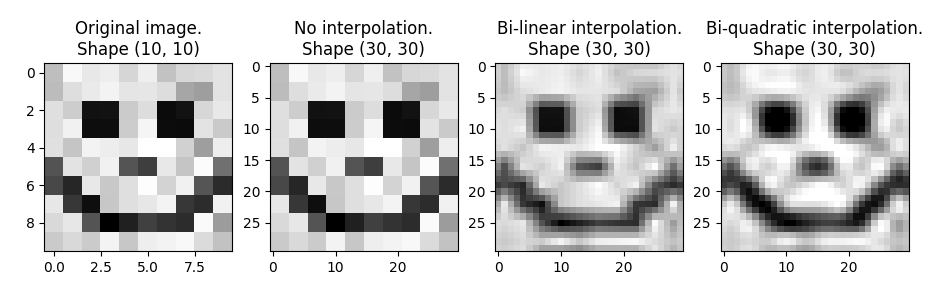
\includegraphics[width=.75\textwidth]{interpolation.png}
		\end{figure}
	}
\end{frame}

\begin{frame}
	{Over- and under-exposure}
	Histograms are a great tool to check the quality of your image. When adjusting the acquisition parameters on a microscope, care should be taken to use as much of the dynamic range as possible to avoid losing information.
	\begin{figure}
		\centering
		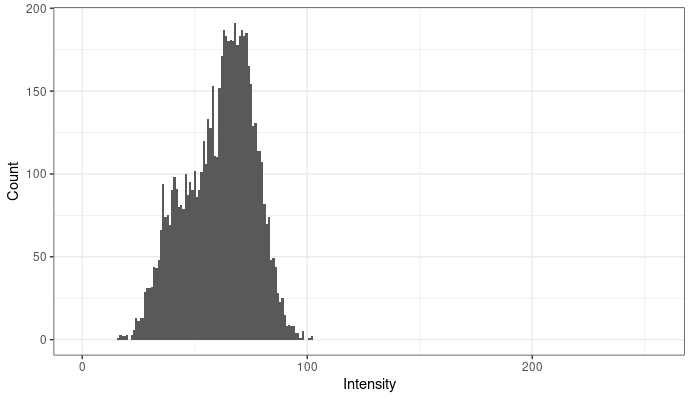
\includegraphics[width=130px]{underexposed.png}
		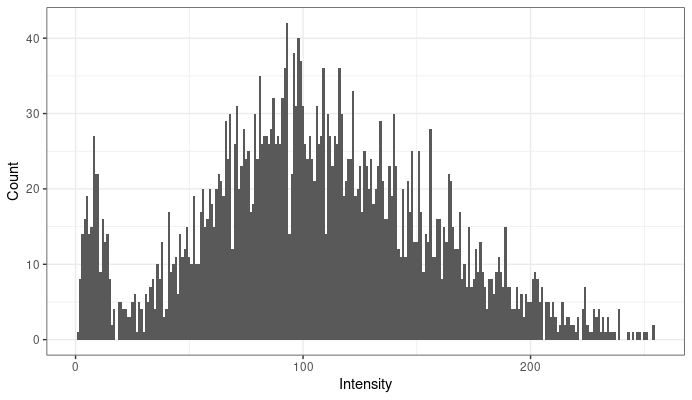
\includegraphics[width=130px]{normalexp.png}
		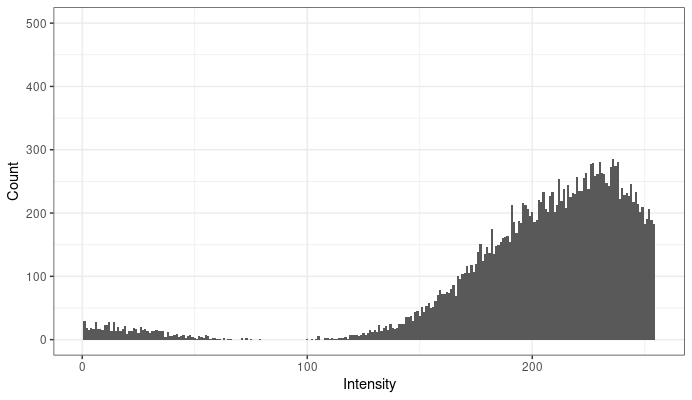
\includegraphics[width=130px]{overexposed.png}
	\end{figure}
\end{frame}

\begin{frame}
	{Histogram manipulation - stretching}
	We can increase the contrast of our image by increasing the amount of dynamic range used by its pixels.

	So, if the pixels in an 8-bit image are between 0 and 50, we are not using the possible information between 50 and 255.

	\pause

	The simplest way of solving this problem without retaking the image is to stretch the histogram.

	If we have an image with intensity limits $m_{im}$ and $M_{im}$, and want to stretch its histogram to $m_{str}$ and $M_{str}$ we can apply the following pixel-wise

	\huge
	$I_{out} = (I_{in} - m_{im})(\frac{M_{str}-m_{str}}{M_{im}-m_{im}} + m_{str})$
\end{frame}

\begin{frame}
	{Histogram stretching in skimage}

	Luckily for us, \textit{skimage.exposure} has a function for that!

	\only<1-2>
	{
		\begin{codebox}
			\texttt{import numpy as np\\
				from skimage import exposure\\
				img = imread("nuclei.tif")\\
				img\_rescale = exposure.rescale\_intensity(img, in\_range=(0, 100))
			}
		\end{codebox}

		\pause
		Often we specify the input range dynamically, for instance by using intensity percentiles

		\begin{codebox}
			\texttt{p2, p98 = np.percentile(img, (2, 98))\\
				img\_rescale = exposure.rescale\_intensity(img, in\_range=(p2, p98))}
		\end{codebox}
	}
	\only<3>{
		\begin{figure}
			\centering
			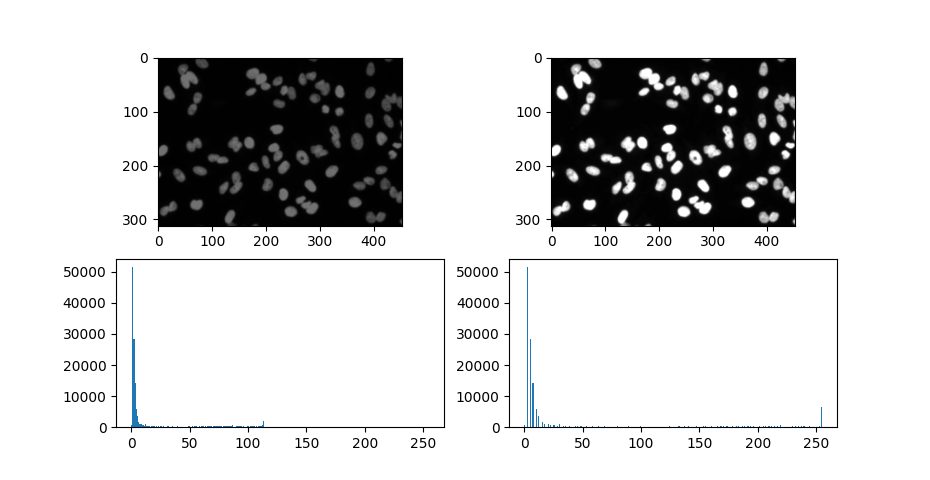
\includegraphics[width=\textwidth]{hist_stretching.png}
		\end{figure}
	}

\end{frame}
\begin{frame}
	{Histogram manipulation - equalization}
	\textbf{Histogram equalization} is a histogram manipulation technique that allows increasing image contrast by spreading the most common intensity values in the image in the possible intensity range.
	\pause
	It does so by flattening the cumulative density function (CDF) of the histogram.

	Given the probability of a pixel to have intensity i (with i between 0 and the maximum pixel value M)\\

	\huge
	$p_x(i) = p(x=i) = \frac{n_i}{n},\quad 0 \le i < M$
	\pause

	\normalsize
	\vspace{2em}
	The CDF is defined as\\

	\huge
	$\text{CDF} = \sum_{j=0}^i p_x(x=j)$
\end{frame}

\begin{frame}
	{Histogram equalization in Python}
	\begin{codebox}
		\texttt{from skimage.exposure import equalize\_hist\\
			img = imread("cells.tif")\\
			img\_eq = equalize\_hist(img)
		}
	\end{codebox}

	\only<1>{
		\begin{figure}
			\centering
			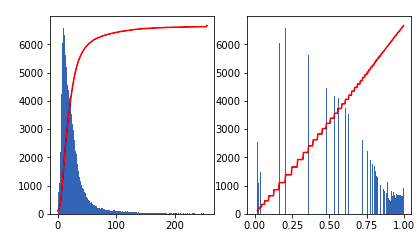
\includegraphics[width=.7\textwidth]{equalisedhisto.png}
		\end{figure}
	}
	\only<2>{
		\begin{figure}
			\centering
			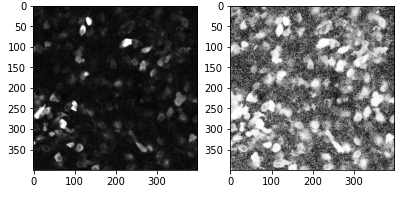
\includegraphics[width=0.7\textwidth]{noise_eq_histo.png}
			\caption{Equalization strengthens signals... but can also increase noise!}
		\end{figure}
	}
\end{frame}

\begin{frame}
	{Better equalization}
	Other more sophisticated equalization strategies exist, such as \textbf{adaptive histogram equalization} (AHE) which computes several histograms of different regions of the image to improve local contrast. This tends to increase noise in areas with low contrast.\\
	\vspace{2em}
	\pause
	\textbf{Contrast Limited Adaptive Equalization} (CLAHE) solves this by reducing the amount of contrast enhancement.\\
	This is implemented in the \texttt{skimage.exposure.equalize\_adapthist} function.
\end{frame}

\begin{frame}
	{Other preprocessing operations}
	Depending on the image and type of analysis you are working on, there are several other operations that can be performed, such as removing noise, blurring or sharpening the image, detecting edges etc.

	These can be obtained by \textbf{convolution} of the image with a \textbf{kernel}.

	\textbf{Convolution} takes each pixel of the image, together with its neighbours, and adds them together weighting the sum by the value of a \textbf{kernel} of the same size of the neighbourhood.

	\pause
	The kernel can be of arbitrary size, and its values should generally sum to 1.
\end{frame}

\begin{frame}
	{Convolution example}
	\only<1>{
		\begin{figure}
			\centering
			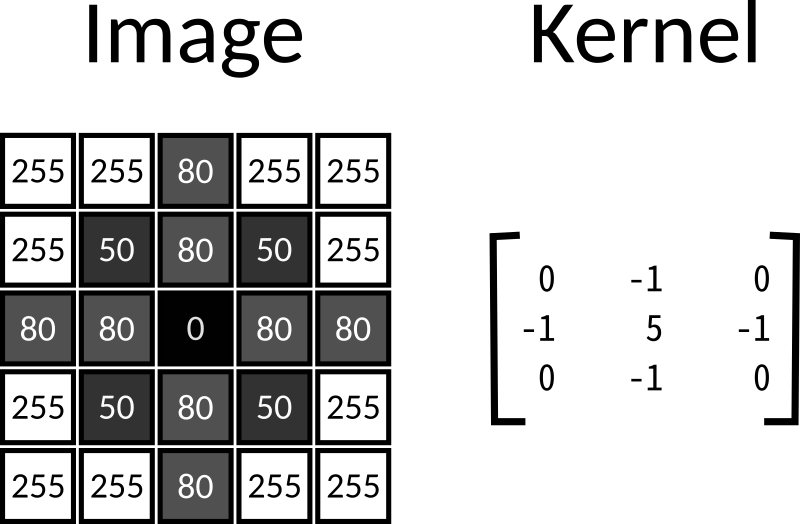
\includegraphics[width=.6\textwidth]{image_kernel.png}
		\end{figure}
	}
	\only<2-3>{
		\begin{figure}
			\centering
			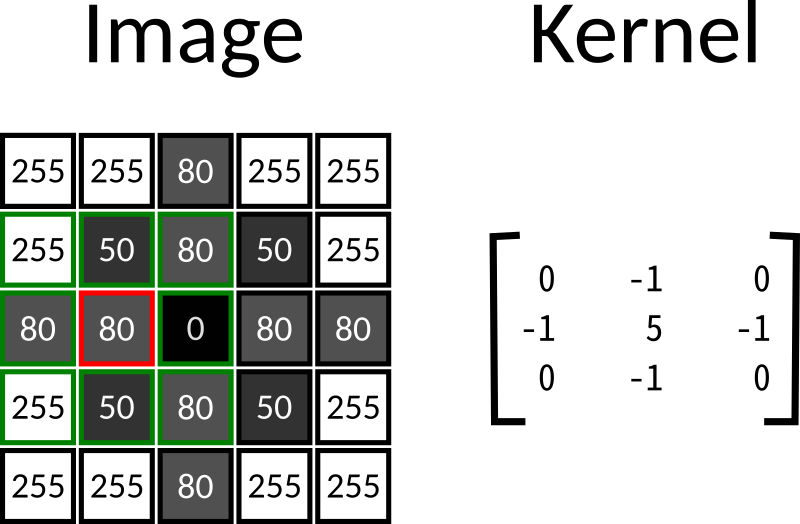
\includegraphics[width=.6\textwidth]{image_kernel_sel.png}
		\end{figure}
		\pause
		The convolved pixel value will be\\
		\Large
		$255 * 0 + 50 * (-1) + 80 * 0 + 80 * (-1) + 80 * 5 + 0 * (-1) + 255 * 0 + 50 * (-1) + 80 * 0 = \mathbf{220}$
	}
	\only<4->{
		\begin{figure}
			\centering
			
\includegraphics[width=.6\textwidth]{filter_before_after.png}
			\caption{Our image after applying the kernel to every pixel.}
			\pause
			Pixel on the edges can be treated in different manner, for example they could be skipped, or the image could be "wrapped around", the kernel cropped... many other solutions exist!

			You can play around with filters on \href{https://setosa.io/ev/image-kernels/}{the "Explained Visually" website}.
		\end{figure}
	}
\end{frame}

\begin{frame}
	{Filters in skimage}
	Scikit Image provides many filters out-of-the-box in the \textit{filters} submodule.
	We will have a look at the most commonly used ones
\end{frame}

\begin{frame}
	{Gaussian blur filter}
	This convolves the image with a Gaussian kernel, which results in stronger contribution of each pixel summed with a weaker contribution from its neighbours, thus resulting in the blurring of the image.

	\only<1>{
		\begin{figure}
			\centering
			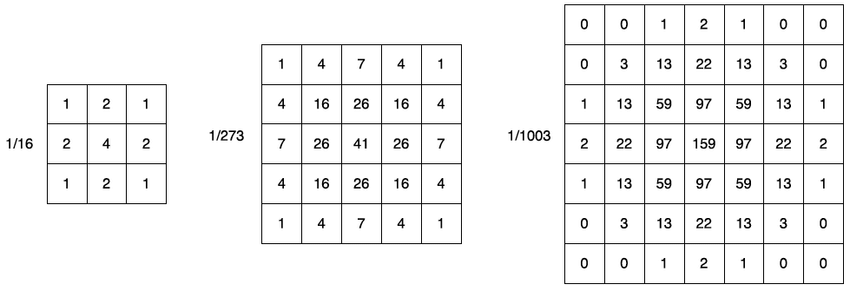
\includegraphics[width=.8\textwidth]{gaussian_kernels.png}
			\caption{3x3, 5x5 and 7x7 Gaussian Kernels}
		\end{figure}
	}

	\only<2->{
		\begin{codebox}
			\texttt{from skimage.filters import gaussian\\
				img = imread("cells.tif")\\
				\# Gaussian filter with kernel size of 3\\
				img\_blur = gaussian(img, 3)}
		\end{codebox}
		\begin{figure}
			\centering
			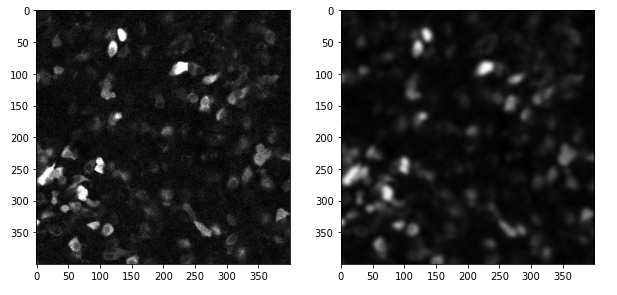
\includegraphics[width=.6\textwidth]{cellsblur.png}
		\end{figure}
	}
\end{frame}

\begin{frame}
	{Sobel filter}
	The Sobel filter is used for edge detection. It uses two kernels, one for determining horizontal edges and one for vertical edges
	\only<1>
	{
		\begin{figure}
			\centering
			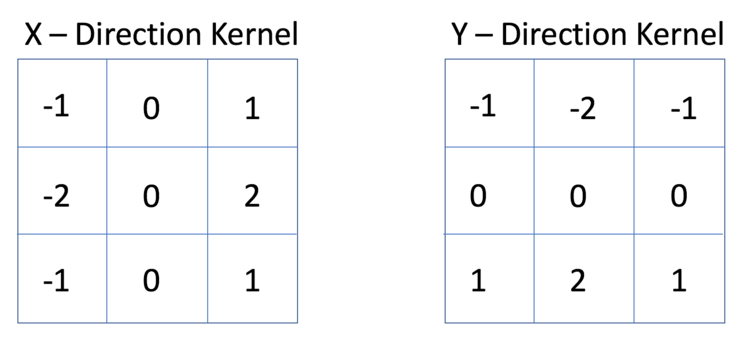
\includegraphics[width=.5\textwidth]{sobel_kernels.png}
		\end{figure}
	}

	\only<2->{
		\begin{codebox}
			\texttt{from skimage.filters import sobel\\
				img = imread("cells.tif")\\
				img\_edges = sobel(img)}
		\end{codebox}
		\begin{figure}
			\centering
			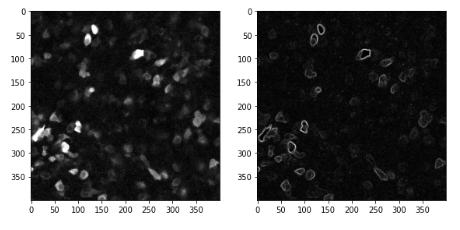
\includegraphics[width=.7\textwidth]{cellsedges.png}
		\end{figure}
	}
\end{frame}

\begin{frame}
	{Median filter}
	The median filter is a commonly used denoising filter. It does not use a convolution kernel, but returns the median value in a $n\times n$ window around each pixel.
	Other denoising filters are available in the \texttt{skimage.restoration} submodule.
	\pause
	\begin{codebox}
		\texttt{from skimage.filters import median\\
			img = imread("cell.tif")\\
			\# Find the median in the 3x3 neighbourhood of
			\# each pixel.\\
			img\_med = median(img, np.ones((3, 3))
		}
	\end{codebox}
	\begin{figure}
		\centering
		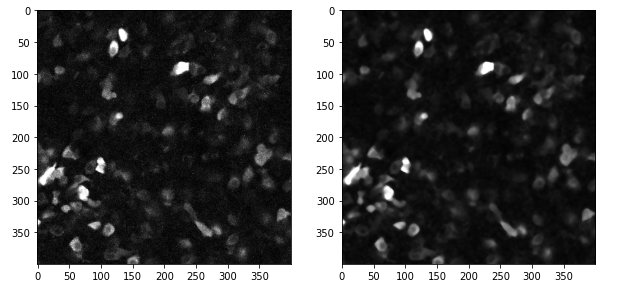
\includegraphics[width=.6\textwidth]{cellsmedian.png}
	\end{figure}
\end{frame}
\end{document}